% !TEX encoding = UTF-8 Unicode
\documentclass[11pt, a4paper]{article}

\usepackage{todonotes}
\usepackage{subcaption}

% Setup of packages used
\usepackage[onehalfspacing]{setspace}		% One half spacing
\newlength{\stockheight}					% To prevent hyperref warning
\setlength{\stockheight}{\paperheight}		% define \stockheigh
\usepackage{hyperref}					% Hyperlinks on pdf (Should be called before Geometry)
\usepackage[a4paper, 					% Page Layout
                     %showframe,				% This shows the frame
                     includehead,
                     footskip=7mm, headsep=6mm, headheight=4.8mm,
                     marginparsep=2mm, marginparwidth=22mm,
                     top=25mm, bottom=25mm, inner=30mm, outer=25mm]{geometry}
\usepackage{sansmathfonts}				% Sans Serif equations
\usepackage[T1]{fontenc}					% Output font encoding for internationa

\usepackage[utf8]{inputenc}			% Encoding of files: utf8
\renewcommand*\familydefault{\sfdefault} 	% Sans Serif as default font
\usepackage{titlesec}					% Redefine chapter and chapter* titles
\titleformat{\chapter}[display]{\huge \bfseries}{\vspace{-0.5cm}\hfill \chaptertitlename\ \thechapter}{0pt}{\hfill}[{\titlerule[1.2pt]}]
\titleformat{name=\chapter,numberless}[display]{\huge \bfseries}{\vspace{-0.5cm}}{0pt}{\hfill}[{\titlerule[1.2pt]}]

% This is used to include the page number on footer within the same margins
%\titleformat{\chapter}[display]{\huge \bfseries}{\vspace{-0.5cm}\hfill \chaptertitlename\ \thechapter}{0pt}{\hfill}[{\titlerule[1.2pt] \enlargethispage{-0.75\baselineskip}}]
%\titleformat{name=\chapter,numberless}[display]{\huge \bfseries}{\vspace{-0.5cm}}{0pt}{\hfill}[{\titlerule[1.2pt] \enlargethispage{-0.75\baselineskip}}]


\usepackage{fancyhdr}					% Package to redefine headers
\fancyhf{}								% No header nor footer
\fancyhead[L]{\thepage}				% Left even and right odd Page Number
\pagestyle{fancy}

\fancypagestyle{plain}{					% To change the footer on chapter and chapter*
	\fancyhf{}							% No header nor footer
%	\fancyfoot[C]{\vspace{-11mm}\thepage}	% Footer with number displaced
	\renewcommand{\headrulewidth}{0pt}	% No line on header
	\renewcommand{\footrulewidth}{0pt}		% No line on footer
}

\RequirePackage{caption} 				% Caption customization
\captionsetup{justification=centerlast,font=small,labelfont=sc,margin=1cm}

\hypersetup{
    colorlinks=true,
    linkcolor=blue,
    filecolor=magenta,      
    urlcolor=blue,
    citecolor=blue,    
}

% Setup the language and its properties (choose only one)
\usepackage[spanish, es-tabla, es-nodecimaldot]{babel}
\addto\captionsspanish{\renewcommand{\contentsname}{Contenido}}
%\usepackage[english]{babel}
%\addto\captionsenglish{\renewcommand{\contentsname}{Contents}}


%\graphicspath{ {figs/} }					% Use this if custom figures folder is needed

\usepackage{amssymb,amsmath}
\usepackage[square, numbers]{natbib}		% Bibliography
\usepackage{tikz}						% Required for title page
\usetikzlibrary{babel}						% Required to make TikZ works with babel
\usepackage[section]{placeins}				% To flush floats before new section
\usepackage{longtable}					% Used by List of Symbols and friends
\usepackage{array}						% Needed by longtable package
\usepackage{graphicx}

%para el color del texto
\usepackage{color}

%para poder poner H en imagenes
\usepackage{float}

%para poder importar excel
\usepackage{csvsimple}
\usepackage{booktabs}

%Para dibujar circuitos
\usepackage{circuitikz}
\usepackage{graphicx}
\usepackage{subcaption}
\usepackage{tikz}
\usetikzlibrary{matrix,calc}
% Macros provided
\def\fecha{\ifcase\month\or
  Enero\or Febrero\or Marzo\or Abril\or Mayo\or Junio\or
  Julio\or Agosto\or Septiembre\or Octubre\or Noviembre\or Diciembre\fi \space\number\year
}
\newcommand*{\subtitle}[1]{\gdef\subtitle{#1}}
\newcommand*{\group}[1]{\gdef\group{#1}}
\newcommand*{\profesor}[1]{\gdef\profesor{#1}}



%%%%%%%%%%%%%%%%%%%%%%karnaugh%%%%%%%%%%%%%%%%%%%%%%%%%


\newcommand{\implicantsol}[3][0]{
    \draw[rounded corners=3pt, fill=#3, opacity=0.3] ($(#2.north west)+(135:#1)$) rectangle ($(#2.south east)+(-45:#1)$);
    }

%internal group
%#1 - Optional. Space between node and grouping line. Default=0
%#2 - top left node
%#3 - bottom right node
%#4 - filling color
\newcommand{\implicant}[4][0]{
    \draw[rounded corners=3pt, fill=#4, opacity=0.3] ($(#2.north west)+(135:#1)$) rectangle ($(#3.south east)+(-45:#1)$);
    }

%group lateral borders
%#1 - Optional. Space between node and grouping line. Default=0
%#2 - top left node
%#3 - bottom right node
%#4 - filling color
\newcommand{\implicantcostats}[4][0]{
    \draw[rounded corners=3pt, fill=#4, opacity=0.3] ($(rf.east |- #2.north)+(90:#1)$)-| ($(#2.east)+(0:#1)$) |- ($(rf.east |- #3.south)+(-90:#1)$);
    \draw[rounded corners=3pt, fill=#4, opacity=0.3] ($(cf.west |- #2.north)+(90:#1)$) -| ($(#3.west)+(180:#1)$) |- ($(cf.west |- #3.south)+(-90:#1)$);
}

%group top-bottom borders
%#1 - Optional. Space between node and grouping line. Default=0
%#2 - top left node
%#3 - bottom right node
%#4 - filling color
\newcommand{\implicantdaltbaix}[4][0]{
    \draw[rounded corners=3pt, fill=#4, opacity=0.3] ($(cf.south -| #2.west)+(180:#1)$) |- ($(#2.south)+(-90:#1)$) -| ($(cf.south -| #3.east)+(0:#1)$);
    \draw[rounded corners=3pt, fill=#4, opacity=0.3] ($(rf.north -| #2.west)+(180:#1)$) |- ($(#3.north)+(90:#1)$) -| ($(rf.north -| #3.east)+(0:#1)$);
}

%group corners
%#1 - Optional. Space between node and grouping line. Default=0
%#2 - filling color
\newcommand{\implicantcantons}[2][0]{
    \draw[rounded corners=3pt, opacity=.3] ($(rf.east |- 0.south)+(-90:#1)$) -| ($(0.east |- cf.south)+(0:#1)$);
    \draw[rounded corners=3pt, opacity=.3] ($(rf.east |- 8.north)+(90:#1)$) -| ($(8.east |- rf.north)+(0:#1)$);
    \draw[rounded corners=3pt, opacity=.3] ($(cf.west |- 2.south)+(-90:#1)$) -| ($(2.west |- cf.south)+(180:#1)$);
    \draw[rounded corners=3pt, opacity=.3] ($(cf.west |- 10.north)+(90:#1)$) -| ($(10.west |- rf.north)+(180:#1)$);
    \fill[rounded corners=3pt, fill=#2, opacity=.3] ($(rf.east |- 0.south)+(-90:#1)$) -|  ($(0.east |- cf.south)+(0:#1)$) [sharp corners] ($(rf.east |- 0.south)+(-90:#1)$) |-  ($(0.east |- cf.south)+(0:#1)$) ;
    \fill[rounded corners=3pt, fill=#2, opacity=.3] ($(rf.east |- 8.north)+(90:#1)$) -| ($(8.east |- rf.north)+(0:#1)$) [sharp corners] ($(rf.east |- 8.north)+(90:#1)$) |- ($(8.east |- rf.north)+(0:#1)$) ;
    \fill[rounded corners=3pt, fill=#2, opacity=.3] ($(cf.west |- 2.south)+(-90:#1)$) -| ($(2.west |- cf.south)+(180:#1)$) [sharp corners]($(cf.west |- 2.south)+(-90:#1)$) |- ($(2.west |- cf.south)+(180:#1)$) ;
    \fill[rounded corners=3pt, fill=#2, opacity=.3] ($(cf.west |- 10.north)+(90:#1)$) -| ($(10.west |- rf.north)+(180:#1)$) [sharp corners] ($(cf.west |- 10.north)+(90:#1)$) |- ($(10.west |- rf.north)+(180:#1)$) ;
}

%Empty Karnaugh map 4x4
\newenvironment{Karnaugh}%
{
\begin{tikzpicture}[baseline=(current bounding box.north),scale=0.8]
\draw (0,0) grid (4,4);
\draw (0,4) -- node [pos=0.7,above right,anchor=south west] {ab} node [pos=0.7,below left,anchor=north east] {cd} ++(135:1);
%
\matrix (mapa) [matrix of nodes,
        column sep={0.8cm,between origins},
        row sep={0.8cm,between origins},
        every node/.style={minimum size=0.3mm},
        anchor=8.center,
        ampersand replacement=\&] at (0.5,0.5)
{
                       \& |(c00)| 00         \& |(c01)| 01         \& |(c11)| 11         \& |(c10)| 10         \& |(cf)| \phantom{00} \\
|(r00)| 00             \& |(0)|  \phantom{0} \& |(1)|  \phantom{0} \& |(3)|  \phantom{0} \& |(2)|  \phantom{0} \&                     \\
|(r01)| 01             \& |(4)|  \phantom{0} \& |(5)|  \phantom{0} \& |(7)|  \phantom{0} \& |(6)|  \phantom{0} \&                     \\
|(r11)| 11             \& |(12)| \phantom{0} \& |(13)| \phantom{0} \& |(15)| \phantom{0} \& |(14)| \phantom{0} \&                     \\
|(r10)| 10             \& |(8)|  \phantom{0} \& |(9)|  \phantom{0} \& |(11)| \phantom{0} \& |(10)| \phantom{0} \&                     \\
|(rf) | \phantom{00}   \&                    \&                    \&                    \&                    \&                     \\
};
}%
{
\end{tikzpicture}
}

%Empty Karnaugh map 2x4
\newenvironment{Karnaughvuit}%
{
\begin{tikzpicture}[baseline=(current bounding box.north),scale=0.8]
\draw (0,0) grid (4,2);
\draw (0,2) -- node [pos=0.7,above right,anchor=south west] {AB} node [pos=0.7,below left,anchor=north east] {C} ++(135:1);
%
\matrix (mapa) [matrix of nodes,
        column sep={0.8cm,between origins},
        row sep={0.8cm,between origins},
        every node/.style={minimum size=0.3mm},
        anchor=4.center,
        ampersand replacement=\&] at (0.5,0.5)
{
                      \& |(c00)| 00         \& |(c01)| 01         \& |(c11)| 11         \& |(c10)| 10         \& |(cf)| \phantom{00} \\
|(r00)| 0             \& |(0)|  \phantom{0} \& |(1)|  \phantom{0} \& |(3)|  \phantom{0} \& |(2)|  \phantom{0} \&                     \\
|(r01)| 1             \& |(4)|  \phantom{0} \& |(5)|  \phantom{0} \& |(7)|  \phantom{0} \& |(6)|  \phantom{0} \&                     \\
|(rf) | \phantom{00}  \&                    \&                    \&                    \&                    \&                     \\
};
}%
{
\end{tikzpicture}
}
\usepackage{multirow}

%Empty Karnaugh map 2x2
\newenvironment{Karnaughquatre}%
{
\begin{tikzpicture}[baseline=(current bounding box.north),scale=0.8]
\draw (0,0) grid (2,2);
\draw (0,2) -- node [pos=0.7,above right,anchor=south west] {a} node [pos=0.7,below left,anchor=north east] {b} ++(135:1);
%
\matrix (mapa) [matrix of nodes,
        column sep={0.8cm,between origins},
        row sep={0.8cm,between origins},
        every node/.style={minimum size=0.3mm},
        anchor=2.center,
        ampersand replacement=\&] at (0.5,0.5)
{
          \& |(c00)| 0          \& |(c01)| 1  \\
|(r00)| 0 \& |(0)|  \phantom{0} \& |(1)|  \phantom{0} \\
|(r01)| 1 \& |(2)|  \phantom{0} \& |(3)|  \phantom{0} \\
};
}%
{
\end{tikzpicture}
}

%Defines 8 or 16 values (0,1,X)
\newcommand{\contingut}[1]{%
\foreach \x [count=\xi from 0]  in {#1}
     \path (\xi) node {\x};
}

%Places 1 in listed positions
\newcommand{\minterms}[1]{%
    \foreach \x in {#1}
        \path (\x) node {1};
}

%Places 0 in listed positions
\newcommand{\maxterms}[1]{%
    \foreach \x in {#1}
        \path (\x) node {0};
}

%Places X in listed positions
\newcommand{\indeterminats}[1]{%
    \foreach \x in {#1}
        \path (\x) node {X};
}





%%%%%%%%%%%%%%%%%%%%%%end karnaugh%%%%%%%%%%%%%%%%%%%%%%








\begin{document}
% !TEX encoding = UTF-8 Unicode
% !TEX root = ../thesis.tex
\title{TRABAJO PR\'ACTICO N\textsuperscript{\underline{o}}2}
\group{Grupo II}
\author{ \newline Pablo Mart\'in  \textsc{Scheinfeld} (59065), \newline
Santiago Agustín \textsc{Arribere} (59169), \newline
Matías Santiago \textsc{Francois} (59828), \newline
Rafael Nicolás \textsc{Trozzo} (59434), \newline
Gonzalo Joaquín \textsc{Davidov} (59117)}

\profesor{\newline Kevin \textsc{Dewald}, \newline
Pablo Enrique  \textsc{Wundes}, \newline
Miguel \textsc{Aguirre}}
\date{\fecha}
\begin{titlepage}
	\onehalfspacing
	\enlargethispage{0.65\baselineskip}
	\begin{tikzpicture}[remember picture, overlay]
		\coordinate (top_right) at 
		    ([xshift=-2.5cm, yshift=-2.5cm]current page.north east);
		\coordinate (top_left) at 
		    ([xshift=2.3cm, yshift=-1.8cm]current page.north west);
		\coordinate (bottom_right) at 
		    ([xshift=-1.8cm, yshift=1.8cm]current page.south east);
		\node[inner sep=0, anchor=north east] at (top_right) {\href{http://www.itba.edu.ar}{
\includegraphics[height=19mm, trim={180 200 200 200}, clip]{figs/logo_itba.png}}};
		\draw[double, line width = 0.5pt] (top_left) rectangle (bottom_right);
	\end{tikzpicture}
	\par
%	\begin{large}
		\vspace{-1cm}
		\noindent \textbf{22.13 - ELECTR\'ONICA III }\par
		\vspace{4cm}
		\begin{center}
			{\Huge \textbf{Trabajo Practico n3}\par}
			%{\Huge \textbf{\title}\par}
			\vspace{1cm}
			{ \Huge \textbf { Electronica 3 } \par}
			%{\huge \textbf{\@subtitle}\par}
			\vspace{1cm}
			%{\Large \textbf{\@group}\par}
			{\Large \textbf{grupo 2}\par}
		\end{center}
		\vfill
		\noindent \textbf{AUTORES:} \\ Arribere Santiago \\Francois Matias \\ Trozzo Nicolas \\ Scheinfeld Pablo \\ Davidov Gonzalo \par
		\vspace{1cm}
		\noindent \textbf{PROFESORES:} \\ Dewald Kevin \\ Wundes Pablo Enrique\\  Aguirre Miguel\par
		\vspace{1cm}
		\begin{center}
			\textbf{CIUDAD AUTÓNOMA DE BUENOS AIRES}\\
			\textbf{13 de Noviembre}\par
		\end{center}
%	\end{large}
\end{titlepage}
\setcounter{tocdepth}{2}
\tableofcontents
\newpage
\section{Ejercicio 1}
\noindent
En la presente sección se tratará el diseño, construcción y medición de un circuito que controla un sistema de dos bombas de agua en base a las señales enviadas por dos sensores, uno ubicado en la parte superior de un tanque de agua, y el otro ubicado en la parte inferior del mismo. Así las señales de los sensores dominan los ciclos de trabajos de las bombas, de tal forma que las bombas alternen sus ciclos de trabajo.\\
%
De esta manera se procedió a realizar una FSM que permita analizar la lógica detrás del circuito a realizar, así, la FSM que controla al sistema se puede ver en la figura \ref{ej1_fsm}, el mismo está realizado con una maquina de Moore.
%
\begin{figure}[H]
    \centering
    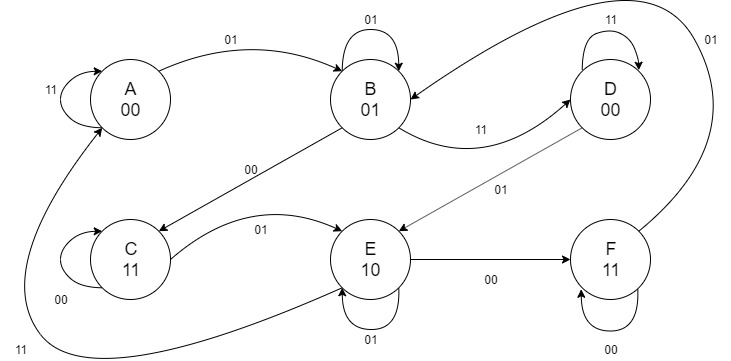
\includegraphics[width=0.7\textwidth]{figs/Ej1/diagrama_grande.jpg} % first figure itself
    \caption{Digrama de estados de la FSM}
    \label{ej1_fsm}
\end{figure}
%
\noindent
De esta manera podemos ver como el diagrama de estados que controla ambas bombas presenta 6 estados, por lo tanto necesitará de al menos 3 flip flop ademas de los componentes lógicos que permitan diseñar la lógica necesaria del sistema. Se consideró por lo tanto que esta solución era ineficiente y por lo tanto se procedió a implementar una FSM de menor tamaño que controle una parte del sistema en cuestión en lugar de todo el sistema como en el caso anterior.\\
Así lo que se realizó fue una FSM que segun las entradas de las señales de los sensores de agua del tanque, entrega 2 salidas posibles, una indica que ambos motores se encuentran encendidos y la otra indica que sólo un motor debe ser encendido. De esta manera luego con ayuda de lógica externa mediante un flip flop T se implementa la lógica correspondiente a la alternancia de los ciclos de trabajo de las bombas.\\
%
Por lo tanto el diagrama de estados correspondiente a este nuevo enfoque del problema se puede ver en la figura \ref{ej1_fsm2}
%
\begin{figure}[H]
    \centering
    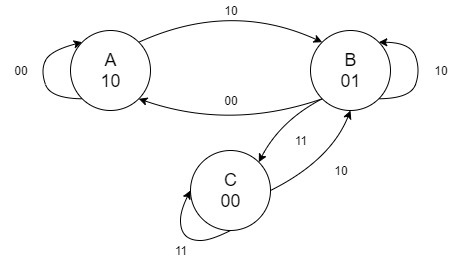
\includegraphics[width=0.7\textwidth]{figs/Ej1/diagrama_chico.jpg} % first figure itself
    \caption{Digrama de estados de la FSM utilizada.}
    \label{ej1_fsm2}
\end{figure}
%
\noindent
Así, la tabla de estados del diagrama se puede ver en la tabla \ref{ej1_tabla}.
%
\begin{table}[H]
\centering
\caption{Tabla de estados.}
\label{ej1_tabla}
\begin{tabular}{|c|c|c|c|c|c|c|}
\hline
\multicolumn{2}{|c|}{Estado Actual}             & \multicolumn{4}{c|}{Estado Siguiente} & Salida                           \\ \hline
\multirow{2}{*}{Nombre} & \multirow{2}{*}{y1y2} & I=0,S=0 & I=0,S=1 & I=1,S=0 & I=1,S=1 & \multirow{2}{*}{Ambas, Solo Una} \\ \cline{3-6}
                        &                       & Y1Y2    & Y1Y2    & Y1Y2    & Y1Y2    &                                  \\ \hline
A                       & 00                    & 00      & XX      & 10      & XX      & 10                               \\ \hline
B                       & 10                    & 00      & XX      & 10      & 11      & 01                               \\ \hline
C                       & 11                    & XX      & XX      & 10      & 11      & 00                               \\ \hline
X                       & 01                    & XX      & XX      & XX      & XX      & XX                               \\ \hline
\end{tabular}
\end{table}
%
\noindent
Así los mapas de karnaugh resultantes se pueden ver a continuación, donde a y b corresponden a y1 e y2 mientras que c y d corresponden a I y S es decir los sensores inferior y superior respectivamente.\\
%
Y1:
\begin{center}
\begin{Karnaugh}
    \minterms{8,10,11,14,15}
    \indeterminats{1,3,4,5,6,7,9,12,13}
    \maxterms{0,2}
    \implicant{12}{10}{red}
\end{Karnaugh}
\end{center}
%
Y2:
\begin{center}
\begin{Karnaugh}
    \minterms{14,15}
    \indeterminats{1,3,4,5,6,7,9,12,13}
    \maxterms{0,2,8,10,11}
    \implicant{4}{14}{green}
\end{Karnaugh}
\end{center}
%
Ambas:
%
\begin{center}
\begin{Karnaughquatre}
    \minterms{0}
    \indeterminats{2}
    \maxterms{1,3}
    \implicant{0}{2}{yellow}
\end{Karnaughquatre}
\end{center}
%
Solo una:
%
\begin{center}
\begin{Karnaughquatre}
    \minterms{1}
    \indeterminats{2}
    \maxterms{0,3}
    \implicantsol{1}{blue}
\end{Karnaughquatre}
\end{center}
%
\noindent
De esta manera las expresiones lógicas resultantes se pueden ver en las ecuaciones \ref{ej1_eq1}.
%
\begin{equation}
\begin{split}
    Y1&=I\\
    Y2&=S\\
    Ambos&=\overline{y1}\\
    Solo\hspace{1mm}uno&=y1\overline{y2}
\label{ej1_eq1}
\end{split}
\end{equation}
\noindent
Por lo que el diagrama del circuito a realizar se puede ver en la figura \ref{ej1_circuito1.}
%
\begin{figure}[H]
    \centering
    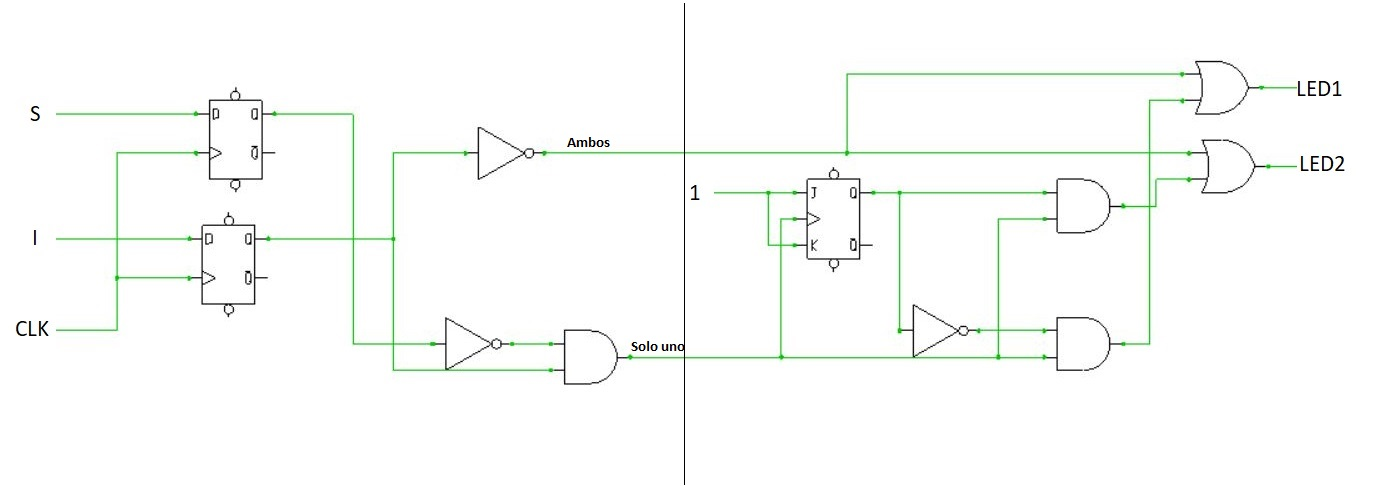
\includegraphics[width=0.9\textwidth]{figs/Ej1/circuitofacilfacil.JPG} % first figure itself
    \caption{Circuito realizado mediante las simplificaciones del mapa de Karnaugh}
    \label{ej1_circuito1.}
\end{figure}
%
\noindent
En el circuito mostrado toda la lógica siguiente a la linea vertical negra corresponde a la utilizada para realizar la alternancia de los ciclos de trabajo de las bombas (LEDS), para ello se utilizó un flip flop JK con la finalidad de construir el Flip flop T necesario del sistema.\\
Se puede notar además en el dibujo de la figura anterior que se puede evitar el uso de ambos flip flop debido a que el sistema no necesita ser sincrónico para funcionar debido a que contempla la entrada asincrónica de las señales de los sensores de los tanques de agua y las salidas asincrónicas de los encendidos de los motores. De todas formas si el sistema requiriese una salida sincrónica porque se conecta con otros sistemas que trabajan de esta forma entonces los flip flops sí serían necesarios. \\
A continuación se muestra el circuito sin el uso de flip flops D.
%
\begin{figure}[H]
    \centering
    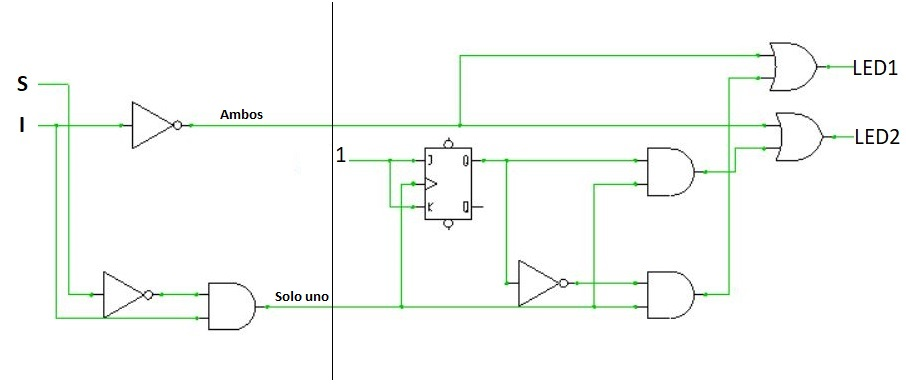
\includegraphics[width=0.9\textwidth]{figs/Ej1/circuito_facil.JPG} % first figure itself
    \caption{Circuito realizado mediante las simplificaciones del mapa de Karnaugh sin los flip flops.}
    \label{ej1_circuito2.}
\end{figure}
%
De esta forma y con la finalidad de ahorrar integrados se realizaron simplificaciones de componentes para lograr utilizar sólo el flip flop jk y compuertan nand, de esta manera el resultado se puede ver en la figura \ref{ej1_circuito3.}.
%
\begin{figure}[H]
    \centering
    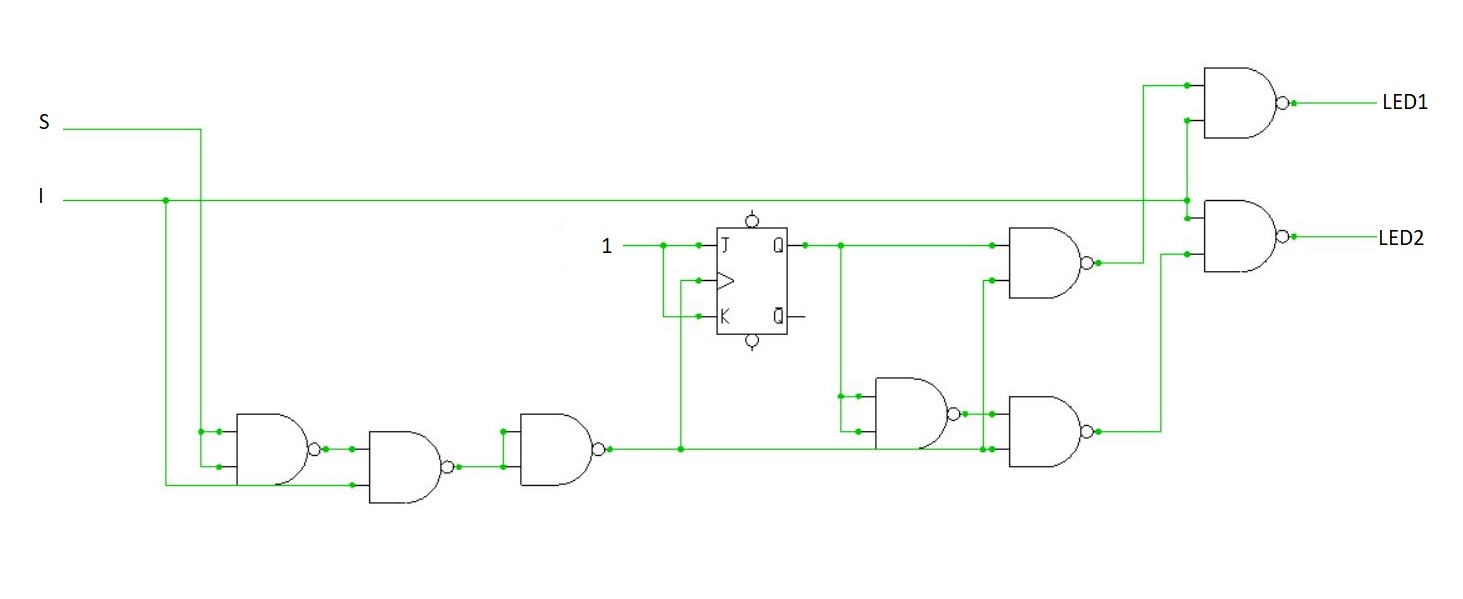
\includegraphics[width=0.9\textwidth]{figs/Ej1/circuito.JPG} % first figure itself
    \caption{Circuito realizado mediante las simplificaciones del mapa de Karnaugh sin los flip flops.}
    \label{ej1_circuito3.}
\end{figure}
%
\noindent
Así, se implementó el circuito en una placa PCB mediante 2 integrados para las compuertas nand, un integrado para el flip flop jk necesario, para las entradas se utilizaron 2 jummpers conectados mediante una resistencia pull down al sistema y a la salida se dispuso de un LED conectado a tierra y al sistema mediante una resistencia que controla la corriente que circula por dicho LED.\\
Los resultados encotrados fueron los esperados, el sistema se comporta fielmente con lo esperado para el mismo.\\
Se anexa en la carpeta de este trabajo un video mostrando el funcionamiento de la placa PCB en cuestión.
\newpage
\section{Ejercicio 2}
\noindent
En la presente sección se planea diseñar e implementar una maquina de estados que analice la secuencia de bits en forma sincrónica de tal forma que encienda una salida cuando reconozca la secuencia de numeros 1-1-0-1 en su entrada.\\
Para ello se utilizará una Máquina de Mealy, de esta manera, se muestra a continuación el diagrama de estados correspondientea a dicha situación en la figura \ref{ej2_estados}
%
\begin{figure}[H]
    \centering
    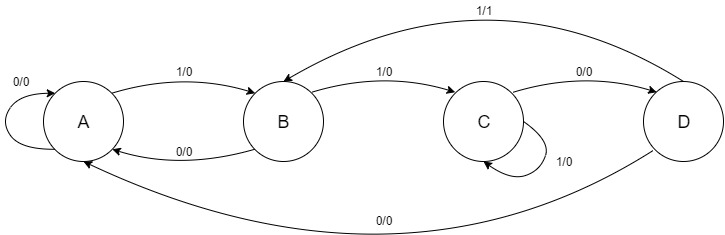
\includegraphics[width=0.8\textwidth]{figs/Ej2/diag_estados.jpg} % first figure itself
    \caption{Diagrama de estados del circuito a realizar.}
    \label{ej2_estados}
\end{figure}
%
De esta manera, la tabla de transisciones queda de la forma de la tabla \ref{ej2_tabla1}.
%
\begin{table}[H]
\caption{Tabla de Estados.}
\label{ej2_tabla1}
\centering
\begin{tabular}{|c|c|c|c|c|c|}
\hline
\multicolumn{2}{|c|}{Estado Actual}             & \multicolumn{2}{c|}{Estado Siguiente} & \multicolumn{2}{c|}{Salida}                 \\ \hline
\multirow{2}{*}{Nombre} & \multirow{2}{*}{y2y1} & W=0               & W=1               & \multirow{2}{*}{W=0} & \multirow{2}{*}{W=1} \\ \cline{3-4}
                        &                       & Y2Y1              & Y2Y1              &                      &                      \\ \hline
A                       & 00                    & 00                & 01                & 0                    & 0                    \\ \hline
B                       & 01                    & 00                & 11                & 0                    & 0                    \\ \hline
C                       & 11                    & 10                & 11                & 0                    & 0                    \\ \hline
D                       & 10                    & 00                & 01                & 0                    & 1                    \\ \hline
\end{tabular}
\end{table}
%
 \noindent
 Así, los mapas de Karnaugh a realizar se pueden ver a continuación, donde A,B,C son y2, y1, W respectivamente.\\
Y1:
%
\begin{center}
    \begin{Karnaughvuit}
       \minterms{4,5,6,7}
        \maxterms{0,1,2,3}
       \implicant{4}{6}{red}
    \end{Karnaughvuit}
\end{center}
%
Y2:
%
\begin{center}
    \begin{Karnaughvuit}
       \minterms{5,7,3}
        \maxterms{0,1,2,4,6}
       \implicant{5}{7}{blue}
       \implicant{3}{7}{green}
    \end{Karnaughvuit}
\end{center}
%
Z:
%
\begin{center}
    \begin{Karnaughvuit}
       \minterms{6}
        \maxterms{0,1,2,3,4,5,7}
        \implicantsol{6}{purple}
    \end{Karnaughvuit}
\end{center}
%
\noindent
Así de esta forma las ecuaciones que se encuentran a partir de los mapas de kernaugh mostrados se pueden ver en las ecuaciones \ref{ej2_eq}.
%
\begin{equation}
\begin{split}
    Y1&=W\\
    Y2&=y1\cdot W+y1\cdot y2 = y1(W+y2)\\
    Z&=y2\cdot \overline{y1}\cdot W
\label{ej2_eq}
\end{split}
\end{equation}
%
Así se puede llegar al circuito de la figura \ref{ej2_circuito.}.
%
\begin{figure}[H]
    \centering
    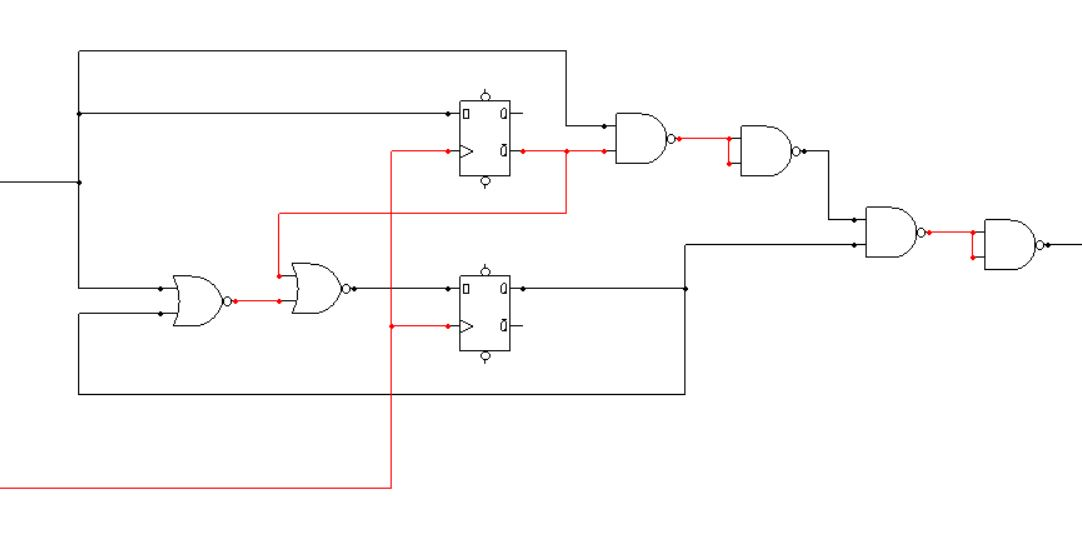
\includegraphics[width=0.8\textwidth]{figs/Ej2/circuit_ej2.JPG} % first figure itself
    \caption{Imagen esquemática del circuito realizado.}
    \label{ej2_circuito.}
\end{figure}
%
Luego se pasó a medir el circuito, para ello se comprobó que todas las secuencias lógicas funcionen de forma correcta al ser testeadas las mismas.\\
De esta manera se procede a mostrar los resultados de las mediciones tomadas para el circuito en cuestión.\\
Para comenzar se muestran en la figura \ref{ej2_resultados1} cómo la salida se activa al detectar el circuito la secuencia de numeros deseado.\\
En verse se puede ver el clock, en violeta la entrada del sistema y en amarillo la salida del mismo.
%
\begin{figure}[H]
    \centering
    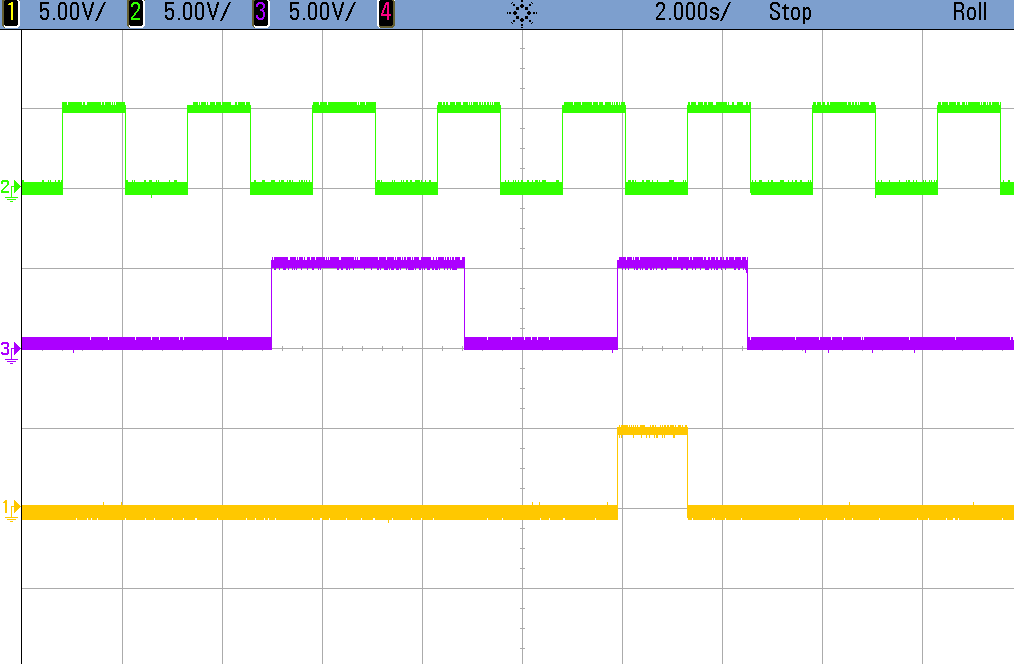
\includegraphics[width=0.6\textwidth]{figs/Ej2/scope_14.png} % first figure itself
    \caption{Mediciones tomadas del circuito, donde se ve como la salida se activa al entrar la secuencia buscada, 1-1-0-1.}
    \label{ej2_resultados1}
\end{figure}
%
Luego en la imagen \ref{ej2_resultados2} se puede ver como el sistema responde de acuerdo a lo esperado al entrar con 1-1-0-1-1-0-1.

%
\begin{figure}[H]
    \centering
    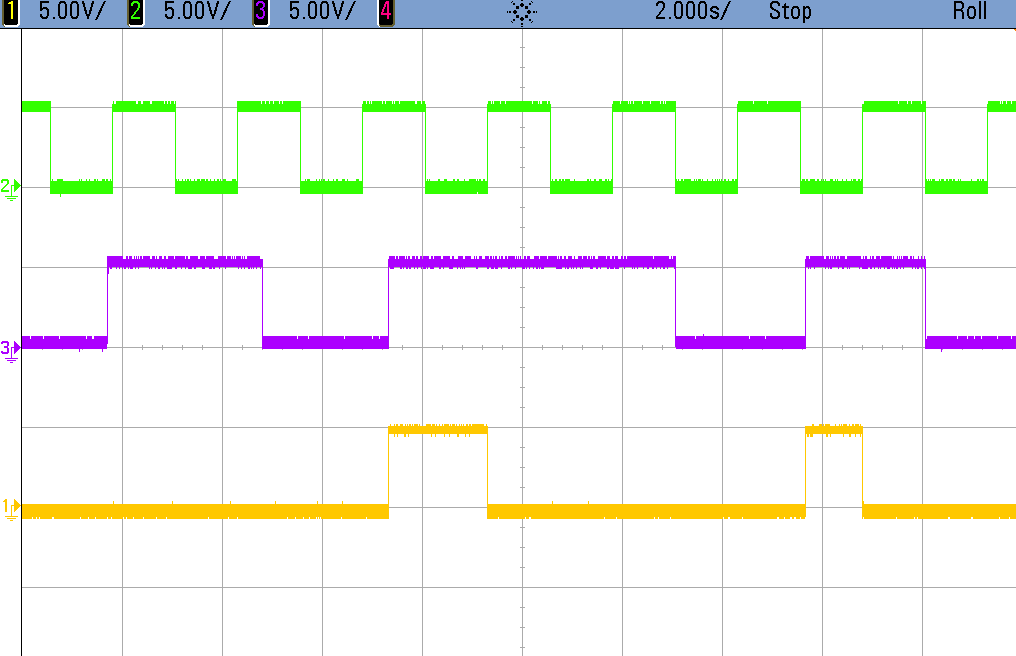
\includegraphics[width=0.6\textwidth]{figs/Ej2/scope_155.png} % first figure itself
    \caption{Mediciones tomadas del circuito, donde se ve como la salida se activa 2 veces con la entrada 1-1-0-1-1-0-1}
    \label{ej2_resultados2}
\end{figure}
%
De esta manera podemos concluir que el circuito funciona de acuerdo a lo esperado, obteniéndose los resultados deseados con el mismo.
\newpage
\section{Ejercicio 3}
En esta sección del presente informe se realizará la implementación fisica de la máquina de Moore que se puede ver en la figura \ref{ej3_diagrama_de_estados}.\\
Para ello se trabajará con entradas de señales de 5V y con lógica interna trabajando con tensiones de 3.3V.
\begin{figure}[H]
    \centering
    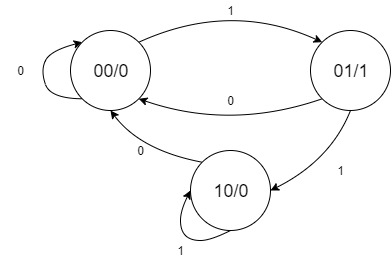
\includegraphics[width=0.6\textwidth]{figs/Ej3/FSM.jpg} % first figure itself
    \caption{Diagrama de estados de Moore a realizar.}
    \label{ej3_diagrama_de_estados}
\end{figure}
%
Así la tabla de estados correspondiente a la situación planteada se puede ver en la tabla \ref{ej3_table1}.
\begin{table}[H]
\caption{Tabla de Estados.}
\label{ej3_table1}
\centering
\begin{tabular}{|c|c|c|c|}
\hline
Estado actual         & \multicolumn{2}{c|}{Estado Siguiente} & Salida             \\ \hline
\multirow{2}{*}{y1y2} & I=0               & I=1               & \multirow{2}{*}{Z} \\ \cline{2-3}
                      & Y2Y1              & Y2Y1              &                    \\ \hline
00                    & 00                & 01                & 0                  \\ \hline
01                    & 00                & 10                & 1                  \\ \hline
10                    & 00                & 10                & 0                  \\ \hline
11                    & XX                & XX                & X                  \\ \hline
\end{tabular}
\end{table}
%
De esta manera los diagramas de Karnaugh del sistema quedan de la siguiente forma, tomando como ABC a y2, y1, I respectivamente.\\
%
Y1:
%
\begin{center}
    \begin{Karnaughvuit}
       \minterms{4}
        \maxterms{0,1,2,5,6}
        \indeterminats{3,7}
       \implicantsol{4}{red}
    \end{Karnaughvuit}
\end{center}
%
Y2:
%
\begin{center}
    \begin{Karnaughvuit}
       \minterms{5,6}
        \maxterms{0,1,2,4}
        \indeterminats{3,7}
       \implicant{5}{7}{green}
        \implicant{7}{6}{blue}
    \end{Karnaughvuit}
\end{center}
%
Z:
%
\begin{center}
    \begin{Karnaughquatre}
       \minterms{2}
        \maxterms{0,1}
        \indeterminats{3}
        \implicant{2}{3}{purple}
    \end{Karnaughquatre}
\end{center}
%
Así, las ecuaciones que se ajustan a los karnaught mostados se pueden ver en las ecuaciones \ref{ej3_eq}.
%
\begin{equation}
\begin{split}
    Y1&=I \cdot \overline{y1} \cdot \overline{y2}\\
    Y2&=y1 \cdot I+y2 \cdot I = (y1 + y2) I\\
    Z&=y1
\label{ej3_eq}
\end{split}
\end{equation}
%
De esta manera el circuito que cumple con estas ecuaciones se puede ver en la figura \ref{ej3_circuito}, en el mismo se decidió por utilizar solo compuertas nand y nor para evitar el uso excesivo de integrados. Ademas se destaca que para el pasaje de 5V a 3.3V se utilizó un diodo zener de 3.3V y una resistencia y para el pasaje de 5V a 3V se utilizó el circuito de la figura \ref{ej3_fig_5v}.
%
\begin{figure}[H]
    \centering
    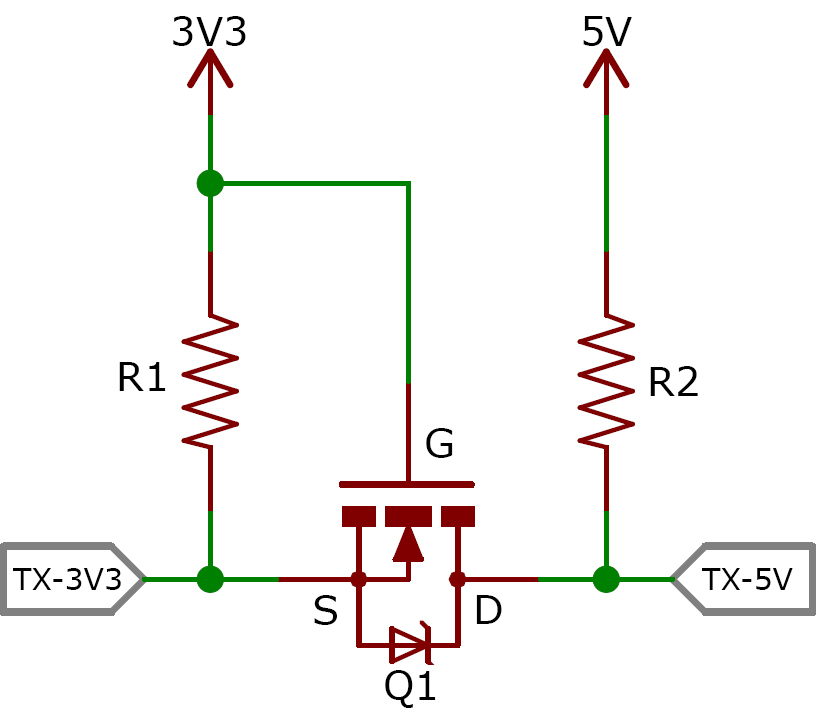
\includegraphics[width=0.3\textwidth]{figs/Ej3/shifter.JPG} % first figure itself
        \caption{Esquema del circuito para convertir 3.3V en 5V}
    \label{ej3_fig_5v}
\end{figure}
%
%
\begin{figure}[H]
    \centering
    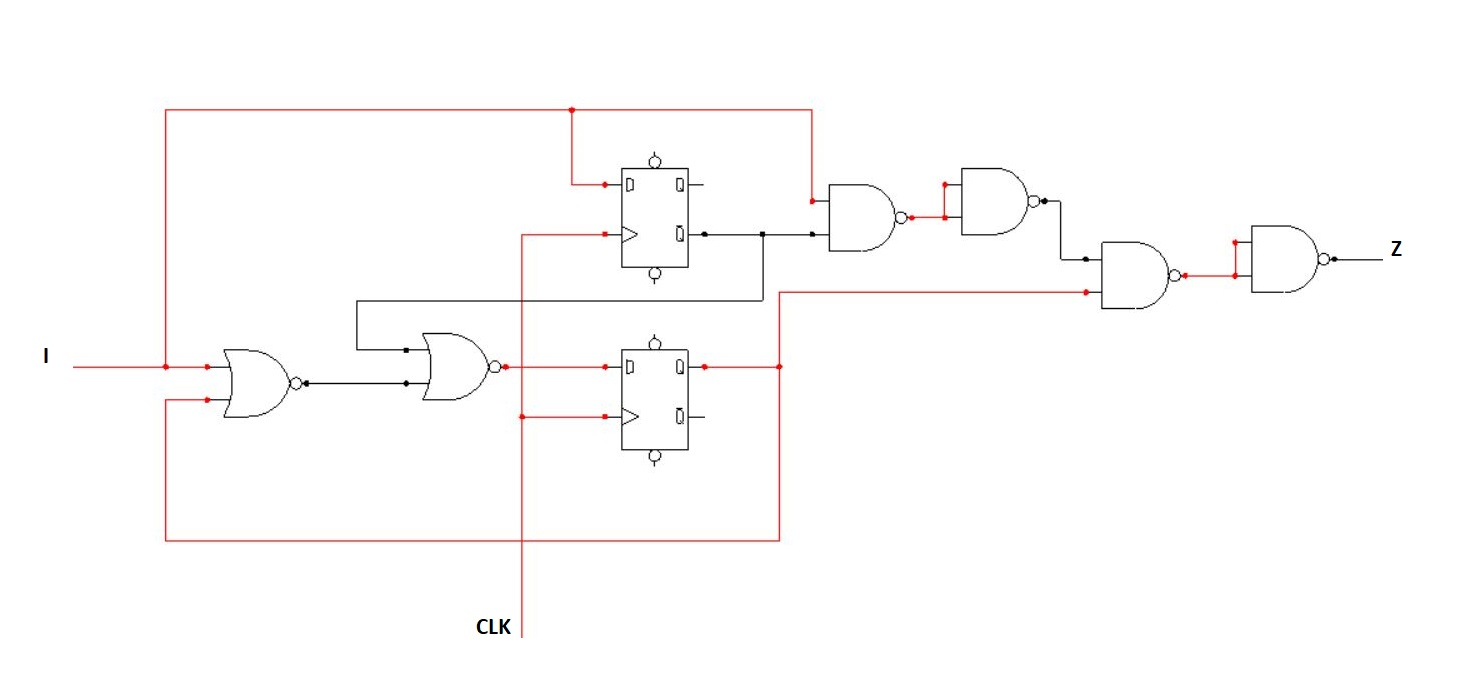
\includegraphics[width=1\textwidth]{figs/Ej3/circ_ej3.JPG} % first figure itself
        \caption{Esquemático del circuito a realizar.}
    \label{ej3_circuito}
\end{figure}
%
De esta manera se implementó el circuito en una placa PCB y se procedió a medir los resultados obtenidos, los mismos se pueden ver en las imagenes \ref{ej3_res1} y \ref{ej3_res2}.
%
\begin{figure}[H]
    \centering
    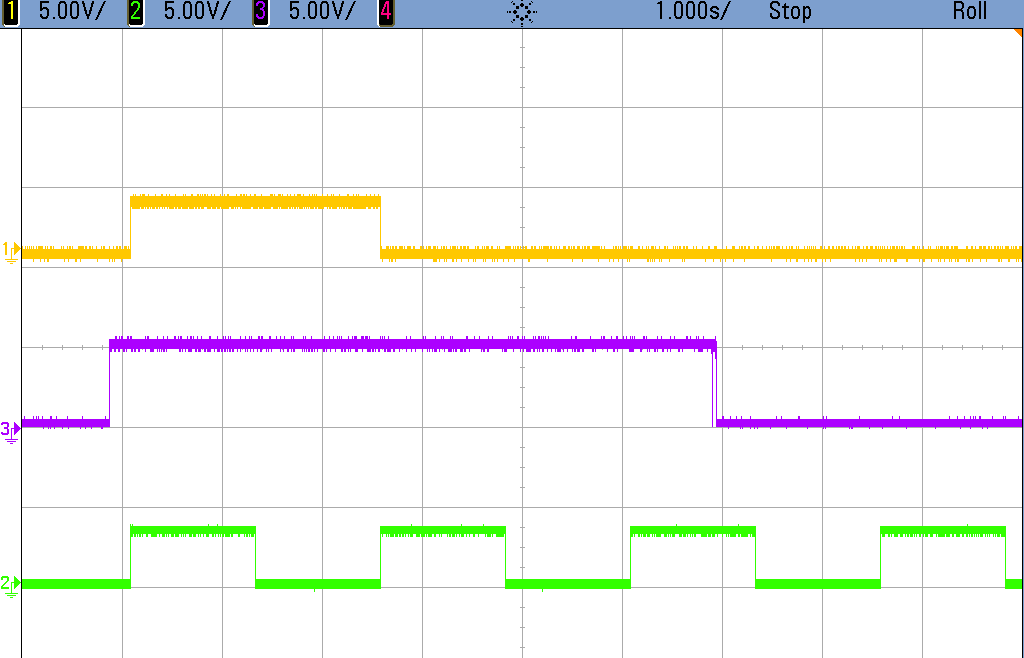
\includegraphics[width=0.6\textwidth]{figs/Ej3/scope_19.png} % first figure itself
        \caption{Respuesta del circuito al entrar con un 1 por mas de un tiempo de clock}
    \label{ej3_res1}
\end{figure}
%
%
\begin{figure}[H]
    \centering
    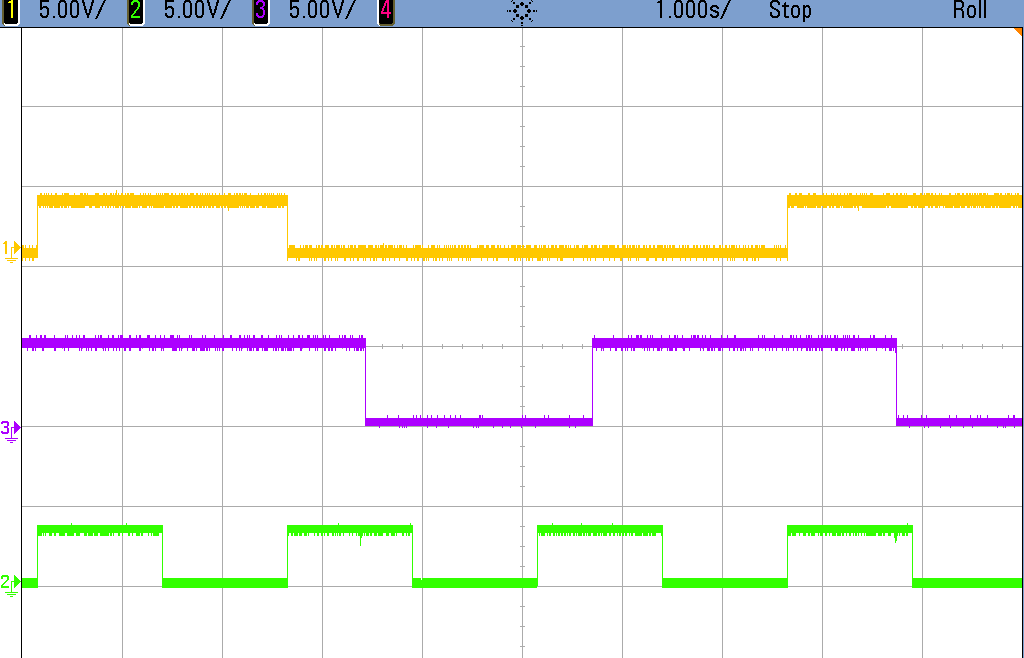
\includegraphics[width=0.6\textwidth]{figs/Ej3/scope_20.png} % first figure itself
        \caption{Respuesta del circuito al entrar dos veces con un uno}
    \label{ej3_res2}
\end{figure}
%
Se puede concluir a partir de las mediciones realizadas que el circuito funciona correctamente y por lo tanto el circuito se comporta como era esperado.
\newpage
\input{sections/conclusion.tex}
\end{document}